\item \textbf{{[}ACJC/PRELIM/9569/2021/P1/Q3{]} }

The diagram below shows a flowchart for performing a search through
a binary tree. The algorithm searches through \texttt{Tree} for \texttt{Searchfor}.
If it finds a node whose data is equal to \texttt{Searchfor}, it outputs
\texttt{Found}. Otherwise, it outputs \texttt{Not Found}.
\noindent \begin{center}
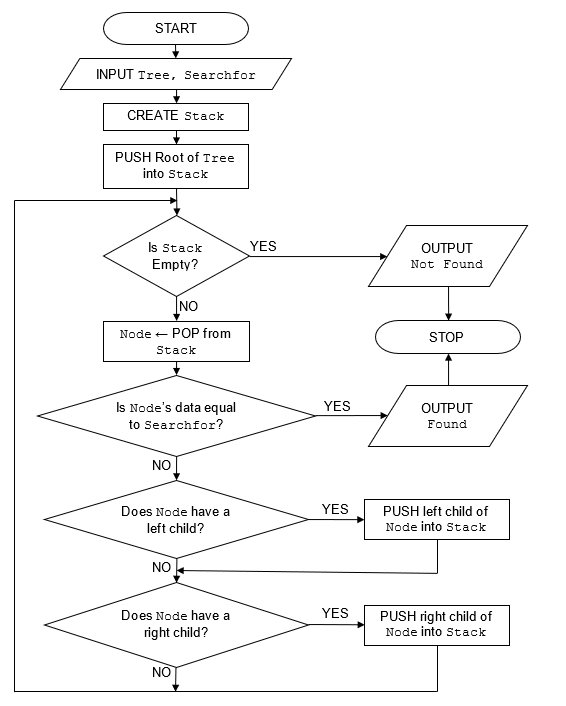
\includegraphics[scale=0.8]{C:/Users/Admin/Desktop/Github/question_bank/LyX/static/img/9569-ACJC-2021-P1-Q3-1}\quad{}
\par\end{center}
\begin{enumerate}
\item Given the input \texttt{Tree} below and a \texttt{Searchfor} value
of 5, draw a trace table to illustrate the algorithm. \hfill{} {[}5{]}
\noindent \begin{center}
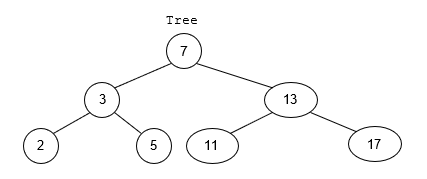
\includegraphics[scale=0.8]{C:/Users/Admin/Desktop/Github/question_bank/LyX/static/img/9569-ACJC-2021-P1-Q3-2}\quad{}
\par\end{center}
\item State whether this is a depth-first search or a breadth-first search.
\hfill{} {[}1{]}
\item Draw a flowchart to illustrate how the other kind of search in (ii)
can be carried out using the same input parameters. \hfill{} {[}3{]}
\item Given the same input \texttt{Tree} and the same \texttt{Searchfo}r
value of 5, draw a trace table to illustrate the algorithm in (iii).
\hfill{} {[}5{]}
\end{enumerate}